\normaltrue \difficilefalse \tdifficilefalse
\correctiontrue

%\UPSTIidClasse{11} % 11 sup, 12 spé
%\newcommand{\UPSTIidClasse}{11}

\exer{Diagramme de Bode $\star\star$ \label{C2:02:510_04}}
\setcounter{question}{0}\marginnote{\xpComp{SLCI}{11}}%\UPSTIcompetence[2]{C2-02}
\index{Compétence C2-02}\index{Compétence SLCI-11}
\index{Diagramme de Bode}
\ifcorrection
\else
\marginnote{\textbf{Pas de corrigé pour cet exercice.}}
\fi




\question{Tracer le diagramme de Bode de la fonction de transfert suivante : 
$F(p)=\dfrac{30}{p^3 + 50,4 p^2 +20 p}$.}


\ifprof

En factorisant, on obtient $F(p)=\dfrac{30}{p\left(p+0,4 \right)\left(p+50 \right)}=\dfrac{40}{20 p\left(\dfrac{p}{0,4}+1 \right)\left(\dfrac{p}{50}+1 \right)}$.
%\textbf{Tracer asymptotique}

%\begin{marginfigure}
%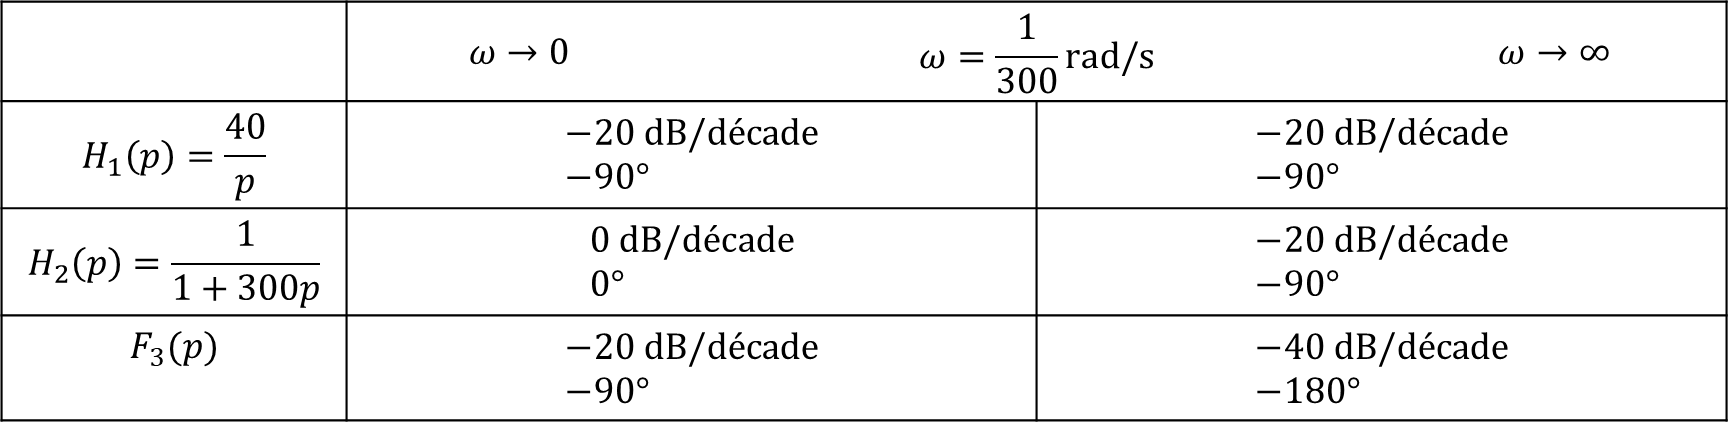
\includegraphics[width=\linewidth]{tab_03}
%\end{marginfigure}
%
%
%\textbf{Positionnement du diagramme de gain}
%Lorsque que $\omega$ tend vers 0, $F_3(p)\simeq \dfrac{40}{p}$. Cette asymptote de pente \SI{-20}{dB/decade} passe par le point $(40,0)$. 


\begin{figure}[!h]
 \begin{tikzpicture}[xscale=2]
\tikzset{
semilog lines/.style={thin, bleuxp}, 
semilog lines 2/.style={semilog lines,bleuxpc},
semilog half lines/.style={semilog lines 2,dotted },
semilog label x/.style={semilog lines,below,font=\tiny,black},
semilog label y/.style={semilog lines,right,font=\tiny,black}
}
\begin{scope}[yscale=1/50]
\semilog{-2}{3}{-160}{50}
\UnitedB
\OrdBode{20}
\BodeAmp[orangexp,thick]{-2:3}{\POAmpAsymp{1.}{2.5}+\POAmpAsymp{1.}{0.02}+\IntAmp{1.5}}%+\POAmpAsymp{100.}{0.083}+\IntAmp{0.01666}}
\BodeAmp[orangexp,ultra thick]{-2:3}{\POAmp{1.}{2.5}+\POAmp{1.}{0.02}+\IntAmp{1.5}}%+\IntAmp{0.01666}}
%\draw (-2.2,27) node {\footnotesize 23,5 dB, 0 dB/d\'ecade};
%\draw (-3.5,120) node {\footnotesize $-$20 dB/d\'ecade};
%\draw (-1.5,65) node {\footnotesize $-$40 dB/d\'ecade};
%\draw [dashed,ultra thick,bleuxp] (-2.47,-1) -- (-2.47,80);
%\draw (-2.47,-1)  node {\Huge $\cdot$} node [above right]{\footnotesize $\dfrac{1}{300}$};
\end{scope}
\begin{scope}[yshift=-5.5cm,yscale=1/90]
\UniteDegre
\OrdBode{45}
\semilog{-2}{3}{-270}{0}
\BodeArg[orangexp,samples=200,thick]{-2:3}{\POArgAsymp{1.}{2.5}+\POArgAsymp{1.}{0.02}+\IntArg{1.5}}
\BodeArg[orangexp,ultra thick]{-2:3}{\POArg{1.}{2.5}+\POArg{1.}{0.02}+\IntArg{1.5}}
\end{scope}
\end{tikzpicture}
\end{figure}

%\begin{marginfigure}
%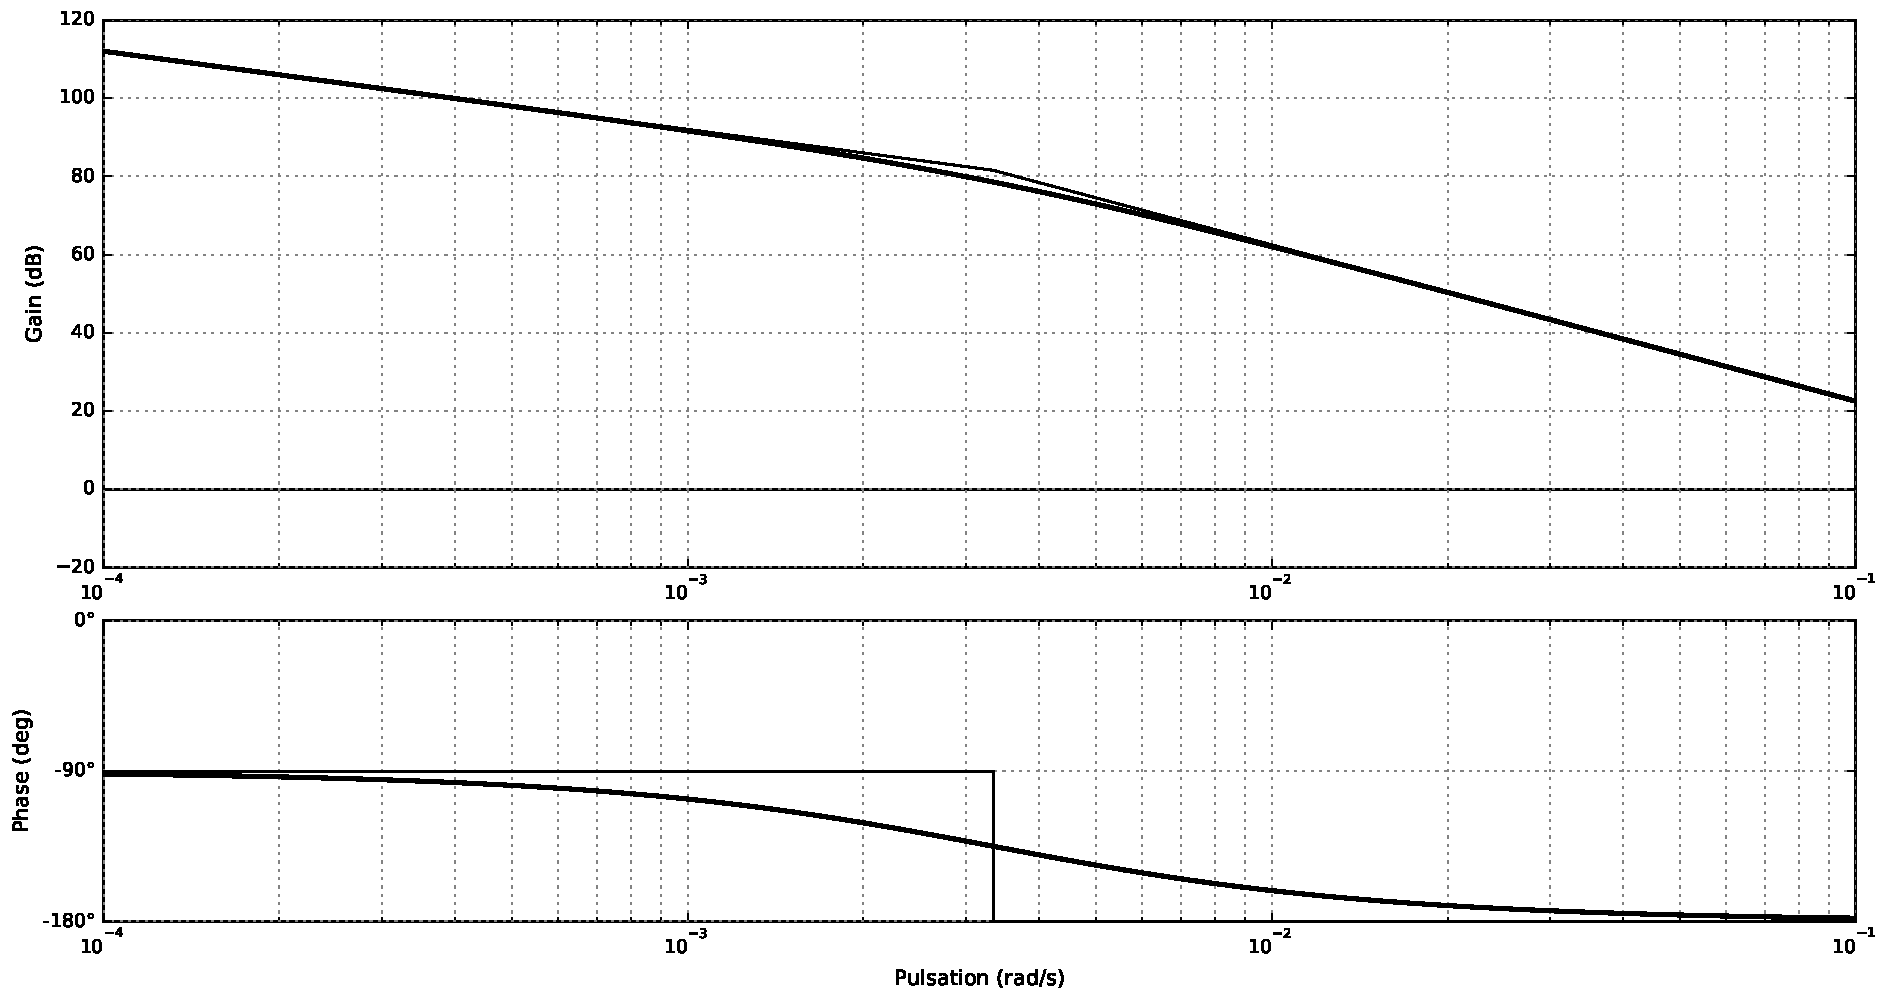
\includegraphics[width=\linewidth]{bode_03}
%\end{marginfigure}

\else 


\begin{figure}[!h]
 \begin{tikzpicture}[xscale=3]
\tikzset{
semilog lines/.style={thin, bleuxp}, 
semilog lines 2/.style={semilog lines,bleuxpc},
semilog half lines/.style={semilog lines 2,dotted },
semilog label x/.style={semilog lines,below,font=\tiny,black},
semilog label y/.style={semilog lines,right,font=\tiny,black}
}
\begin{scope}[yscale=1/60]
\OrdBode{20}
\semilog{-2}{3}{-160}{50}

\end{scope}
\begin{scope}[yshift=-5.5cm,yscale=1/90]
\UniteDegre
\OrdBode{45}
\semilog{-2}{3}{-270}{0}
\end{scope}
\end{tikzpicture}
\end{figure}

%\begin{marginfigure}
%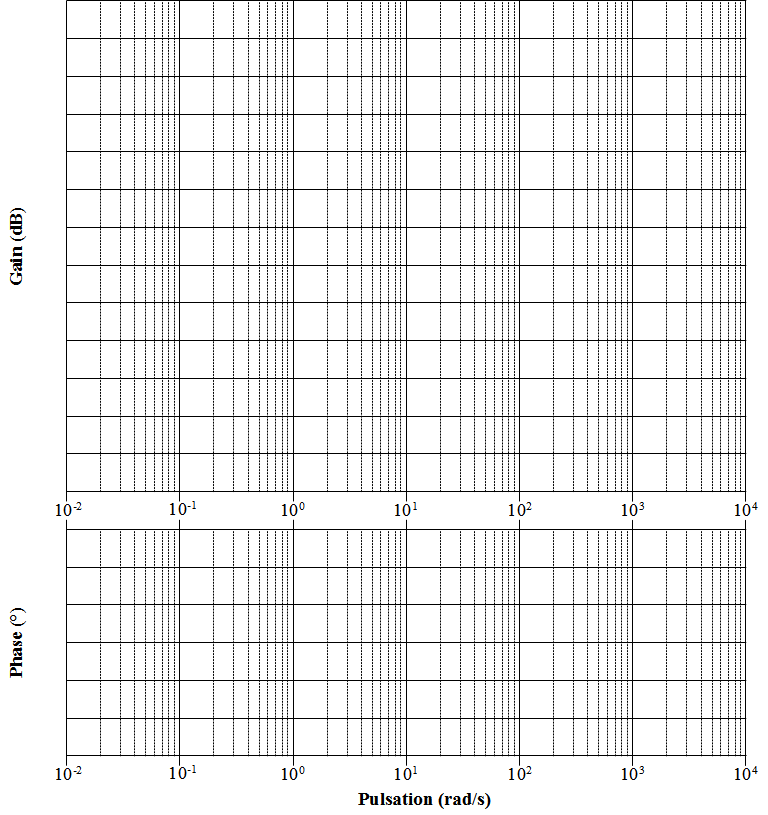
\includegraphics[width=\linewidth]{510_01}
%\end{marginfigure}
\fi





%\question{Réaliser le schéma-blocs.}
%\ifprof
%\begin{figure}[H]
%\centering
%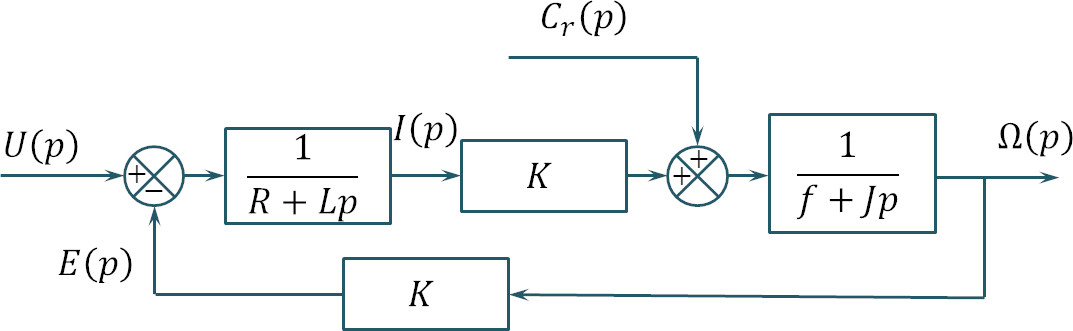
\includegraphics[width=\linewidth]{51_01_c}
%%\caption{Évolution du couple utile en fonction de la vitesse de rotation pour des
%%fréquences de commande de \SI{90}{Hz} à \SI{110}{Hz}. \label{fig_50_04}}
%\end{figure}
%\else
%\fi



\ifprof
\else

\marginnote{Corrigé voir \ref{C2:02:510_04}.}

\fi